\setcounter{chapter}{-1}
\chapter{绪论:量子力学背景}

1900年,Kelvin勋爵给英国皇家研究院做了一个广为人知的演讲,题为《覆盖热和光的动力学理论的十九世纪的乌云》\footnote{\textit{Nineteenth-Century Clouds over the Dynamical Theory of Heat and Light}. }。
\begin{quote}
	The beauty and clearness of the dynamical theory, which asserts heat and light to be modes of motion, is at present obscured by two clouds.
	I. The first came into existence with the undulatory theory of light, and was dealt with by Fresnel and Dr. Thomas Young; it involved the question, How could the earth move through an elastic solid, such as essentially is the luminiferous ether?
	II. The second is the Maxwell-Boltzmann doctrine regarding the partition of energy.
\end{quote}
他所说的两朵\textit{乌云}是指:
\begin{itemize}
    \item 物质如何穿过以太而运动;%\footnote{Michelson-Morley实验};
    \item 统计力学中的能量均分原理可能会被打破。
\end{itemize}
而在二十世纪,针对这两个问题,产生了两个主要的物理理论:针对前者产生了狭义相对论;针对后者产生了量子力学。%\url{https://books.google.com.tw/books?id=YvoAAAAAYAAJ&pg=PA363&redir_esc=y#v=onepage&q&f=false}

涉及统计力学的部分,包括热容、Einstein晶体模型等,详见本人的统计力学笔记内容,此处不多赘述。

\section{黑体辐射问题}

19世纪,人们希望研究物体热辐射的性质,比如通过烧热钢铁的颜色来判断其温度。
为了避免外界辐射的因素,可以考虑一个可以完全吸收外界辐射的理想物体,由于这种物体不反射任何光线,因此称为\textbf{黑体}。
因此,黑体的辐射便完全取决于其本身的性质,比如说温度。

\iffalse
考虑边长为$L$的立方黑体,电磁波在其内满足驻波条件:
\[
	k^2=k_x^2+k_y^2+k_z^2=\kh{\frac\pi{L}}^2\kh{n_x^2+n_y^2+n_z^2}.
\]
其中$k=2\pi/\lambda$为波数,对应频率$\nu=c/\lambda=ck/2\pi$,$n_x,n_y,n_z$是驻波在$x,y,z$方向上的半波长个数,应为不全为0的非负整数。
由上式,解$(n_x,n_y,n_z)$分布在半径为$kL/\pi=2\nu L/c$的球面上,则球内解的个数为
\[
	N(\nu)=2\cdot\frac18\cdot\frac43\pi\kh{\frac{2L\nu}c}^3=\frac{8\pi L^3}{3c^3}\nu^3,
\]
系数前乘2是因为光是横波,存在两种偏振态.
\fi

每个解$(n_x,n_y,n_z)$都对应一种驻波状态,其密度定义为:
\[
	g(\nu)=\frac1{L^3}\dv{N(\nu)}\nu=\frac{8\pi}{c^3}\nu^2.
\]
根据Boltzmann分布,每个状态上的粒子数$\propto\e{-\varepsilon/\kB T}$。
故能量平均值为
\begin{align}
	\avg E=\frac{\textstyle\int\zti\varepsilon\e{-\varepsilon/\kB T}\d\varepsilon}{\textstyle\int\zti\e{-\varepsilon/\kB T}\d\varepsilon}=\kB T.
\end{align}
因此能量密度
\[
u(\nu,T)=\avg Eg(\nu)=\frac{8\pi\nu^2}{c^3}\kB T.
\]
考虑黑体辐射在$4\pi$立体角内是各向同性的,
辐射率\footnote{指定方向上的单位立体角和垂直此方向的单位面积上的辐射通量.}
为
\begin{align}
	\label{eqn:Rayleigh-Jeans Formula of frequency}
	I_\nu(\nu,T)=\frac c{4\pi}u(\nu,T)=\frac{2\nu^2}{c^2}\kB T.
\end{align}
如果以波长$\lambda$为变量,%由于得到$g$的过程中有求导,因此
\begin{align}
	\label{eqn:Rayleigh-Jeans Formula of wavelength}
	I_\lambda(\lambda,T)=\frac{c}{\lambda^2}\cdot I_\nu\biggkh{\frac c\lambda,T}=\frac{2c\kB T}{\lambda^4}.
\end{align}
注意
$I_\nu$的单位为$\si{J/m^2}$,
而$I_\lambda$的单位为$\si{W/m^3}$.

\eqref{eqn:Rayleigh-Jeans Formula of frequency}和\eqref{eqn:Rayleigh-Jeans Formula of wavelength}式被称为Rayleigh-Jeans公式.可以看到,当$\lambda\to0$时,$I_\lambda(\lambda,T)\to\infty$,这显然与事实不符,因此被称为\textit{紫外灾难}.\footnote{需要指出的时间顺序:Rayleigh于1900年推导公式,Jeans于1905年修正系数,紫外灾变是Ehrenfest于1911年提出,而Planck公式提出于1900年.}

\paragraph{能量量子化}

Wein通过对黑体辐射的实验数据进行拟合,提出了一个经验公式:
\begin{equation}
	I_\lambda=C_1\lambda^{-5}\e{-C_2/\lambda T},
\end{equation}
其在$\lambda$较小时符合得很好,但在$\lambda$较大时存在较大偏差。
Planck为了
Planck的解决方法是将能量分布变为离散的,即$\varepsilon_n=nh\nu$
\begin{align}
	\avg E=\frac{\textstyle\sum_{n=1}^\infty \varepsilon_n\e{-\varepsilon_n/\kB T}}{\textstyle\sum_{n=1}^\infty\e{-\varepsilon_n/\kB T}}=\frac{h\nu}{\e{h\nu/\kB T}-1}.
\end{align}
由此得到的辐射率与实验符合的很好。

\begin{center}
	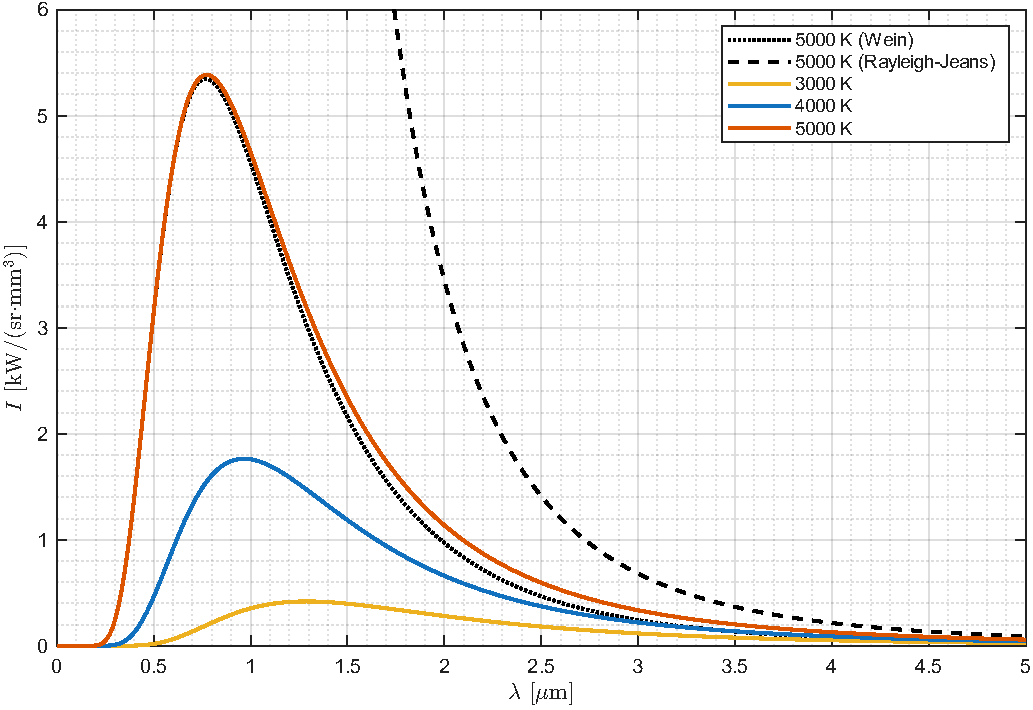
\includegraphics[width=0.8\linewidth]{figures/blackbody.pdf}
	\captionof{figure}{黑体辐射}
	\label{fig:blackbody radiation}
\end{center}

\begin{theorem}{Planck黑体辐射定律}{Planck's Law}
	黑体辐射的辐射率
	\begin{align}
		I_\nu(\nu,T)=\frac{2h\nu^3}{c^2}\frac{1}{\e{h\nu/\kB T}-1}.
	\end{align}
	波长情况下
	\begin{align}
		I_\lambda(\lambda,T)=\frac{2hc^2}{\lambda^5}\frac{1}{\e{hc/\lambda\kB T}-1}
	\end{align}
\end{theorem}
由$x\to0$时,$\e x-1\sim x$,有
\[
	\lambda\gg\frac{hc}{\kB T},\quad I_\lambda\sim\frac{2c\kB T}{\lambda^4}.
\]
正是Rayleigh-Jeans公式的形式.

考虑$I_\lambda(\lambda,T)$最大时对应的波长$\lambda_{\mathrm m}$,做变换$\xi=\frac{hc}{\lambda\kB T}$,则
\begin{align*}
	\dv{I_\lambda}\lambda & =\dv{I_\lambda}\xi\cdot\dv\xi\lambda\propto\dd\xi\biggkh{\frac{\xi^5}{\e\xi-1}}
	=\frac{\xi^4\bigfkh{5(\e\xi-1)-\xi\e\xi}}{(\e\xi-1)^2}=0.
\end{align*}
\iffalse
	\[
		\dv{I_\lambda}\lambda=\frac c4\cdot\frac{8\pi}{3c^3}\cdot\dd\lambda\kh{\frac{h\nu}{\e{h\nu/\kB T}-1}\cdot\dd\lambda\nu^3}.
	\]
	由
	\[
		\dd\lambda=\dd\nu\cdot\dv\nu\lambda=-\frac c{\lambda^2}\dd\nu=-\frac{\nu^2}c\dd\nu.
	\]
	故
	\begin{align*}
		\dv r\lambda&=\frac{2h}{3c^2}\cdot\frac{\nu^2}{c}\cdot\dd\nu\kh{\frac{\nu}{\e{h\nu/\kB T}-1}\cdot\frac{\nu^2}c\cdot 3\nu^2}\\
		&=\frac{2h\nu^2}{c^4}\cdot\dd\nu\frac{\nu^5}{\e{h\nu/\kB T}-1},
	\end{align*}
	设$\xi:=h\nu/\kB T$,则导数等价于
	\[
		\dd\xi\frac{\xi^5}{\e\xi-1}=\frac{\xi^4}{\kh{\e\xi-1}^2}\fkh{5\kh{\e\xi-1}-\xi\e\xi}=0.
\]
\fi
解方程
\[
	\xi=5\bigkh{1-\e{-\xi}}\implies\xi_0=\num{4.96511423}\ldots
\]
\begin{theorem}{Wein位移定律}{Wien's Displacement Law}
	黑体电磁辐射光谱辐射度的峰值波长与自身温度乘积为常数
	\begin{align}
		\lambda_\mathrm m T=\frac{hc}{4.965\kB}=\SI{2.89777}{\mm\K}.
	\end{align}
\end{theorem}
\iffalse
	let $x:=\frac{\lambda kT}{hc}$, then $\d\lambda=\frac{hc}{kT}\d x,\frac{2\pi hc^2}{\lambda^5}=\frac{2\pi k^5T^5}{h^4c^3}\frac1{x^5}$
	\begin{align*}
		\frac{\d r}{\d\lambda} & =\frac{kT}{hc}\frac{2\pi k^5T^5}{h^4c^3}\frac{\d}{\d x}\frac1{x^5(e^{1/x}-1)}     \\
		                       & =\frac{2\pi k^6T^6}{h^5c^4}\frac{5x^4(e^{1/x}-1)+x^3e^{1/x}}{x^{10}(e^{1/x}-1)^2} \\
		                       & =\frac{2\pi k^6T^6}{h^5c^4}\frac{5xe^{1/x}-5x+e^{1/x}}{x^7(e^{1/x}-1)^2}
	\end{align*}
\fi
黑体表面单位面积在单位时间内辐射出的总能量
\[
	j=\int\zti\int_{\Omega_0}I_\nu(\nu,T)\cos\theta\d\Omega\d\nu
\]
黑体辐射几何上严格符合Lambert余弦定律,因此
\begin{align*}
	j & =\int\zti\int_0^{2\pi}\int_0^{\pi/2}I_\nu(\nu,T)\cos\theta\sin\theta\d\theta\d\varphi\d\nu \\
	  & =\pi\int\zti I_\nu(\nu,T)\d\nu=\frac{2\pi h}{c^2}\int\zti\frac{\nu^3}{\e{h\nu/\kB T}-1}\d\nu,
\end{align*}
又
\[
	\int\zti\frac{x^3\d x}{\e x-1}=\Gamma(4)\zeta(4)=3!\times\frac{\pi^4}{90}=\frac{\pi^4}{15},
\]
得到
\begin{theorem}{Stefan-Boltzmann定律}{Stefan-Boltzmann Law}
	黑体表面单位面积在单位时间内辐射出的总能量
	\begin{align}
		j=\sigma T^4.
	\end{align}
	其中$\sigma:=\frac{2\pi^5k^4}{15h^3c^2}=\SI{5.6704e-8}{\W\per\m\squared\per\K\squared}.$
\end{theorem}
\section{光电效应和Compton效应}
1897年,Hertz发现紫外线照射到金属电极上,可以帮助产生电火花。对于光电效应中经典理论所不能解释的现象,1905年\footnote{该年Einstein发布了四篇划时代的论文,分别涉及光电效应、Brown运动、狭义相对论和质能方程,也被称为Einstein奇迹年。}Einstein在他的论文《关于光的产生和转变的一个启发性观点》中主张光子也是量子化的,其能量$E=h\nu$,且光电效应方程
\begin{align}
	\Ek=h\nu-W.
\end{align}
其中$\Ek$为光电子最大初动能,$W$为金属表面逸出功.

1923年,Compton发现X射线跟物质相互作用时,散射光波长变长的现象。利用光子的动量$p=h/\lambda$,得出增加的波长与散射角的关系
\begin{align}
	\D\lambda=\frac h{m_\elc c}\kh{1-\cos\theta}.
\end{align}

这些效应证明了光具有\textbf{波粒二象性}
\begin{align}
	E=h\nu,\quad p=\frac h\lambda.
\end{align}
\section{Bohr原子模型}
1914年,Franck-Hertz实验表明,原子能级是分立的;对氢原子光谱有Rydberg经验公式
\begin{align}
	\frac1\lambda=R_\infty\kh{\frac1{n^2}-\frac1{m^2}}.
\end{align}

1913年,Bohr为了解决氢原子问题,提出电子角动量是量子化的
\begin{align}
	L=m_\elc vr=n\hbar,\quad n=1,2,\ldots
\end{align}
再利用经典力学中,Coulomb力提供电子圆周运动的向心力
\[
	\frac1{4\pi\varepsilon_0}\frac{e^2}{r^2}=m_\elc\frac{v^2}r.
\]
解得电子速率
\begin{align}
	v_n=\frac{e^2}{4\pi\varepsilon_0}\frac{1}{n\hbar}=\frac{e^2}{2nh\varepsilon_0},
\end{align}
特别地,基态电子速率和光速的比值是一个无量纲常数:精细结构常数
\[
	\alpha\equiv\frac{e^2}{2\varepsilon_0 hc}\doteq\frac1{137}.
\]

电子轨道半径
\begin{align}
	r_n=\frac{4\pi\varepsilon_0\hbar^2}{m_\elc e^2}n^2,
\end{align}
称基态半径为Bohr半径
\[
a_0\equiv\frac{4\pi\varepsilon_0\hbar^2}{m_\elc e^2}=\SI{5.29177e-11}{m}.
\]

能量
\begin{align}
	E_n=-\frac{m_\elc e^4}{8\varepsilon_0^2h^2}\frac1{n^2},
\end{align}
基态能量
\[
E_1=-\frac{m_\elc e^3}{8\varepsilon_0^2h^2}e=\SI{-13.6}{\eV}.
\]

由跃迁条件
\[
h\nu=E_n-E_m,
\]
可得Rydberg常数
\[
R_\infty=\frac{m_\elc e^4}{8\varepsilon_0^2h^3c}=\SI{1.09737375e7}{\per\m}.
\]

为处理多自由度体系的周期运动的分立能级问题,Sommerfeld提出了推广的量子化条件,对于周期运动的广义坐标和广义动量$(q,p)$
\begin{align}
	\oint p\d q=nh,\quad n=1,2,\ldots
\end{align}

1924年,de Broglie提出实物粒子也具有波粒二象性:
\[
	\lambda=\frac hp,\quad\nu=\frac Eh.
\]
并称之为物质波,1926年Bohr提出概率波的概念.